% !TeX root = ../thuthesis-example.tex

\chapter{视觉惯性里程计}

本章主要对视觉惯性里程计模块进行介绍。本文中的视觉惯性里程计不同于通用的里程计,其专门针对车辆或者轮式机器人进行了优化,针对这类平台的运动状态进行了假设与分类,并根据分类情况分别提出了相应的速度伪观测约束条件。在状态的检测方面,本章介绍了一种基于深度学习的方法。在约束条件的使用方面,本章设计了粗对齐过程并在原有的后端优化中加入了惯性-车体因子。

\section{整体设计}
视觉惯性里程计是视觉惯性定位中的关键组成部分,其主要工作是为定位提供较为精确的帧间运动关系约束,这对于最终的定位精度有着不可忽视的作用。视觉惯性里程计常用于无人机、自动驾驶车辆和机器人等领域,传统的视觉惯性里程计一般考虑机体做任意运动,因此仅构建了惯性和视觉观测之间的约束关系。而然,在固定路线的定位中,机体的运动往往自身同样具有一定的伪观测约束:本文考虑的汽车和轮式机器人,其运动往往在平面上进行,因此其速度一般可以分解为沿着车辆前进方向的速度和沿着车身横向的速度。如图~\ref{fig:vehicle} 所示,实线代表IMU体坐标系$(\cdot)^{b_{j}}$,虚线代表车身坐标系$(\cdot)^{v_{j}}$,车身坐标系的$y$轴沿着车辆前进方向,$x$轴沿着车辆横向方向,$z$轴垂直于地面向上。IMU体坐标系即IMU的测量坐标系,其一般状态下与车身坐标系会存在一定的旋转关系,并不一定如图所示的共向。

\begin{figure}
  \centering
  \tikzset{every picture/.style={line width=0.75pt}} %set default line width to 0.75pt        
  \begin{tikzpicture}[x=0.75pt,y=0.75pt,yscale=-1,xscale=1]
  %uncomment if require: \path (0,300); %set diagram left start at 0, and has height of 300

  %Image [id:dp3701434269039574] 
  \draw (145,144.74) node  {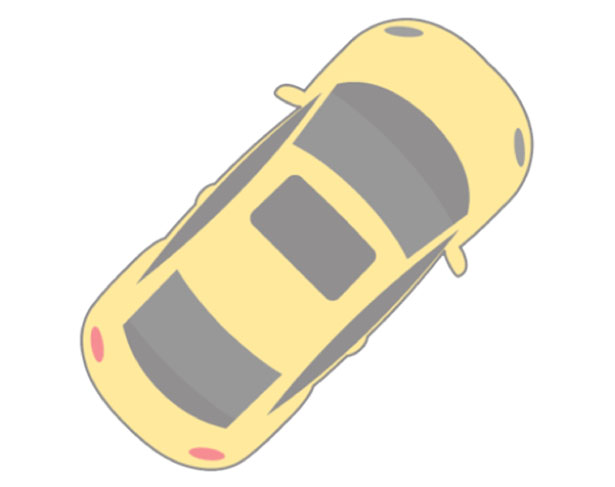
\includegraphics[width=99pt,height=74.61pt]{vehicle.png}};
  %Straight Lines [id:da20058009351259742] 
  \draw [color={rgb, 255:red, 74; green, 144; blue, 226 }  ,draw opacity=1 ][line width=1.5]  [dash pattern={on 5.63pt off 4.5pt}]  (146,146) -- (217.39,111.73) ;
  \draw [shift={(221,110)}, rotate = 154.36] [fill={rgb, 255:red, 74; green, 144; blue, 226 }  ,fill opacity=1 ][line width=0.08]  [draw opacity=0] (10.92,-2.73) -- (0,0) -- (10.92,2.73) -- cycle    ;
  %Straight Lines [id:da5603181046378807] 
  \draw [color={rgb, 255:red, 208; green, 2; blue, 27 }  ,draw opacity=1 ][line width=1.5]  [dash pattern={on 5.63pt off 4.5pt}]  (146,146) -- (195.98,189.38) ;
  \draw [shift={(199,192)}, rotate = 220.96] [fill={rgb, 255:red, 208; green, 2; blue, 27 }  ,fill opacity=1 ][line width=0.08]  [draw opacity=0] (10.92,-2.73) -- (0,0) -- (10.92,2.73) -- cycle    ;
  %Straight Lines [id:da43883225903692824] 
  \draw [color={rgb, 255:red, 65; green, 117; blue, 5 }  ,draw opacity=1 ][line width=1.5]  [dash pattern={on 5.63pt off 4.5pt}]  (146,146) -- (202.29,84.94) ;
  \draw [shift={(205,82)}, rotate = 132.67] [fill={rgb, 255:red, 65; green, 117; blue, 5 }  ,fill opacity=1 ][line width=0.08]  [draw opacity=0] (10.92,-2.73) -- (0,0) -- (10.92,2.73) -- cycle    ;
  %Straight Lines [id:da4769565351313416] 
  \draw [color={rgb, 255:red, 74; green, 144; blue, 226 }  ,draw opacity=1 ][line width=1.5]    (146.28,144.45) -- (221.23,118.89) ;
  \draw [shift={(225.02,117.6)}, rotate = 161.17] [fill={rgb, 255:red, 74; green, 144; blue, 226 }  ,fill opacity=1 ][line width=0.08]  [draw opacity=0] (10.92,-2.73) -- (0,0) -- (10.92,2.73) -- cycle    ;
  %Straight Lines [id:da3562334885093257] 
  \draw [color={rgb, 255:red, 208; green, 2; blue, 27 }  ,draw opacity=1 ][line width=1.5]    (146.28,144.45) -- (190.76,193.45) ;
  \draw [shift={(193.45,196.41)}, rotate = 227.77] [fill={rgb, 255:red, 208; green, 2; blue, 27 }  ,fill opacity=1 ][line width=0.08]  [draw opacity=0] (10.92,-2.73) -- (0,0) -- (10.92,2.73) -- cycle    ;
  %Straight Lines [id:da672459548829603] 
  \draw [color={rgb, 255:red, 65; green, 117; blue, 5 }  ,draw opacity=1 ][line width=1.5]    (146.28,144.45) -- (209.41,90.5) ;
  \draw [shift={(212.45,87.9)}, rotate = 139.48] [fill={rgb, 255:red, 65; green, 117; blue, 5 }  ,fill opacity=1 ][line width=0.08]  [draw opacity=0] (10.92,-2.73) -- (0,0) -- (10.92,2.73) -- cycle    ;
  %Straight Lines [id:da7351111533191295] 
  \draw [color={rgb, 255:red, 65; green, 117; blue, 5 }  ,draw opacity=1 ][line width=1.5]  [dash pattern={on 5.63pt off 4.5pt}]  (286,159) -- (342.29,97.94) ;
  \draw [shift={(345,95)}, rotate = 132.67] [fill={rgb, 255:red, 65; green, 117; blue, 5 }  ,fill opacity=1 ][line width=0.08]  [draw opacity=0] (10.92,-2.73) -- (0,0) -- (10.92,2.73) -- cycle    ;
  %Straight Lines [id:da5481629305422135] 
  \draw [color={rgb, 255:red, 65; green, 117; blue, 5 }  ,draw opacity=1 ][line width=1.5]  [dash pattern={on 1.69pt off 2.76pt}]  (447,152) -- (503.29,90.94) ;
  \draw [shift={(506,88)}, rotate = 132.67] [fill={rgb, 255:red, 65; green, 117; blue, 5 }  ,fill opacity=1 ][line width=0.08]  [draw opacity=0] (10.92,-2.73) -- (0,0) -- (10.92,2.73) -- cycle    ;
  %Straight Lines [id:da7036682415956479] 
  \draw [color={rgb, 255:red, 208; green, 2; blue, 27 }  ,draw opacity=1 ][line width=1.5]  [dash pattern={on 1.69pt off 2.76pt}]  (447,152) -- (468.05,171.3) ;
  \draw [shift={(471,174)}, rotate = 222.51] [fill={rgb, 255:red, 208; green, 2; blue, 27 }  ,fill opacity=1 ][line width=0.08]  [draw opacity=0] (10.92,-2.73) -- (0,0) -- (10.92,2.73) -- cycle    ;
  %Straight Lines [id:da1265383231355004] 
  \draw [color={rgb, 255:red, 245; green, 166; blue, 35 }  ,draw opacity=1 ][line width=1.5]  [dash pattern={on 5.63pt off 4.5pt}]  (447,152) -- (522.51,109.95) ;
  \draw [shift={(526,108)}, rotate = 150.88] [fill={rgb, 255:red, 245; green, 166; blue, 35 }  ,fill opacity=1 ][line width=0.08]  [draw opacity=0] (10.92,-2.73) -- (0,0) -- (10.92,2.73) -- cycle    ;

  % Text Node
  \draw (195,194.4) node [anchor=north west][inner sep=0.75pt]  [font=\footnotesize,color={rgb, 255:red, 208; green, 2; blue, 27 }  ,opacity=1 ]  {$x$};
  % Text Node
  \draw (210,69.4) node [anchor=north west][inner sep=0.75pt]  [font=\footnotesize,color={rgb, 255:red, 65; green, 117; blue, 5 }  ,opacity=1 ]  {$y$};
  % Text Node
  \draw (229,106.4) node [anchor=north west][inner sep=0.75pt]  [font=\footnotesize]  {$\textcolor[rgb]{0.29,0.56,0.89}{z}$};
  % Text Node
  \draw (160,176.4) node [anchor=north west][inner sep=0.75pt]  [font=\large]  {$b_{j}$};
  % Text Node
  \draw (186,155.4) node [anchor=north west][inner sep=0.75pt]  [font=\large]  {$v_{j}$};
  % Text Node
  \draw (249,180) node [anchor=north west][inner sep=0.75pt]   [align=left] {直线行驶速度方向};
  % Text Node
  \draw (418,181) node [anchor=north west][inner sep=0.75pt]   [align=left] {转弯速度方向(黄色)};


  \end{tikzpicture}
  \caption{车身坐标系和IMU体坐标系分解示意}
  \label{fig:vehicle}
\end{figure}

在当前的坐标系下,假设车辆或机器人行驶在平面(不考虑上下坡导致的$z$轴速度),其状态可能存在3种情况:
\begin{enumerate}
  \item 车辆静止,此状态下车身坐标系的$y$与$x$轴均无速度;
  \item 直线行驶,此状态下车身坐标系的$y$轴有速度,$x$轴无速度;
  \item 车辆转弯,此状态下车身坐标系的$y$与$x$轴均有速度。
\end{enumerate}

据此分析,可以在车辆或机器人静止和直线行驶时,可以为车身增加两项伪观测,而这两项伪观测可以作为约束条件提升视觉惯性里程计的精度。但是,在仅依靠IMU信息和视觉信息的情况下,如何区分车辆的运动状态仍是一个有待解决的问题。此外,这两项约束如何添加到原有的视觉惯性里程计的优化中,也需要进一步的研究。未解决上述问题,本文在本章着重介绍如图~\ref{fig:vio_pipeline} 所示的视觉惯性里程计。该视觉惯性里程计在一般设计的基础上加入了车身状态判别、惯性-车体粗对齐等过程,并在窗口优化中加入了惯性-车体因子,以上改动以绿色标注。

\begin{figure}
  \centering
  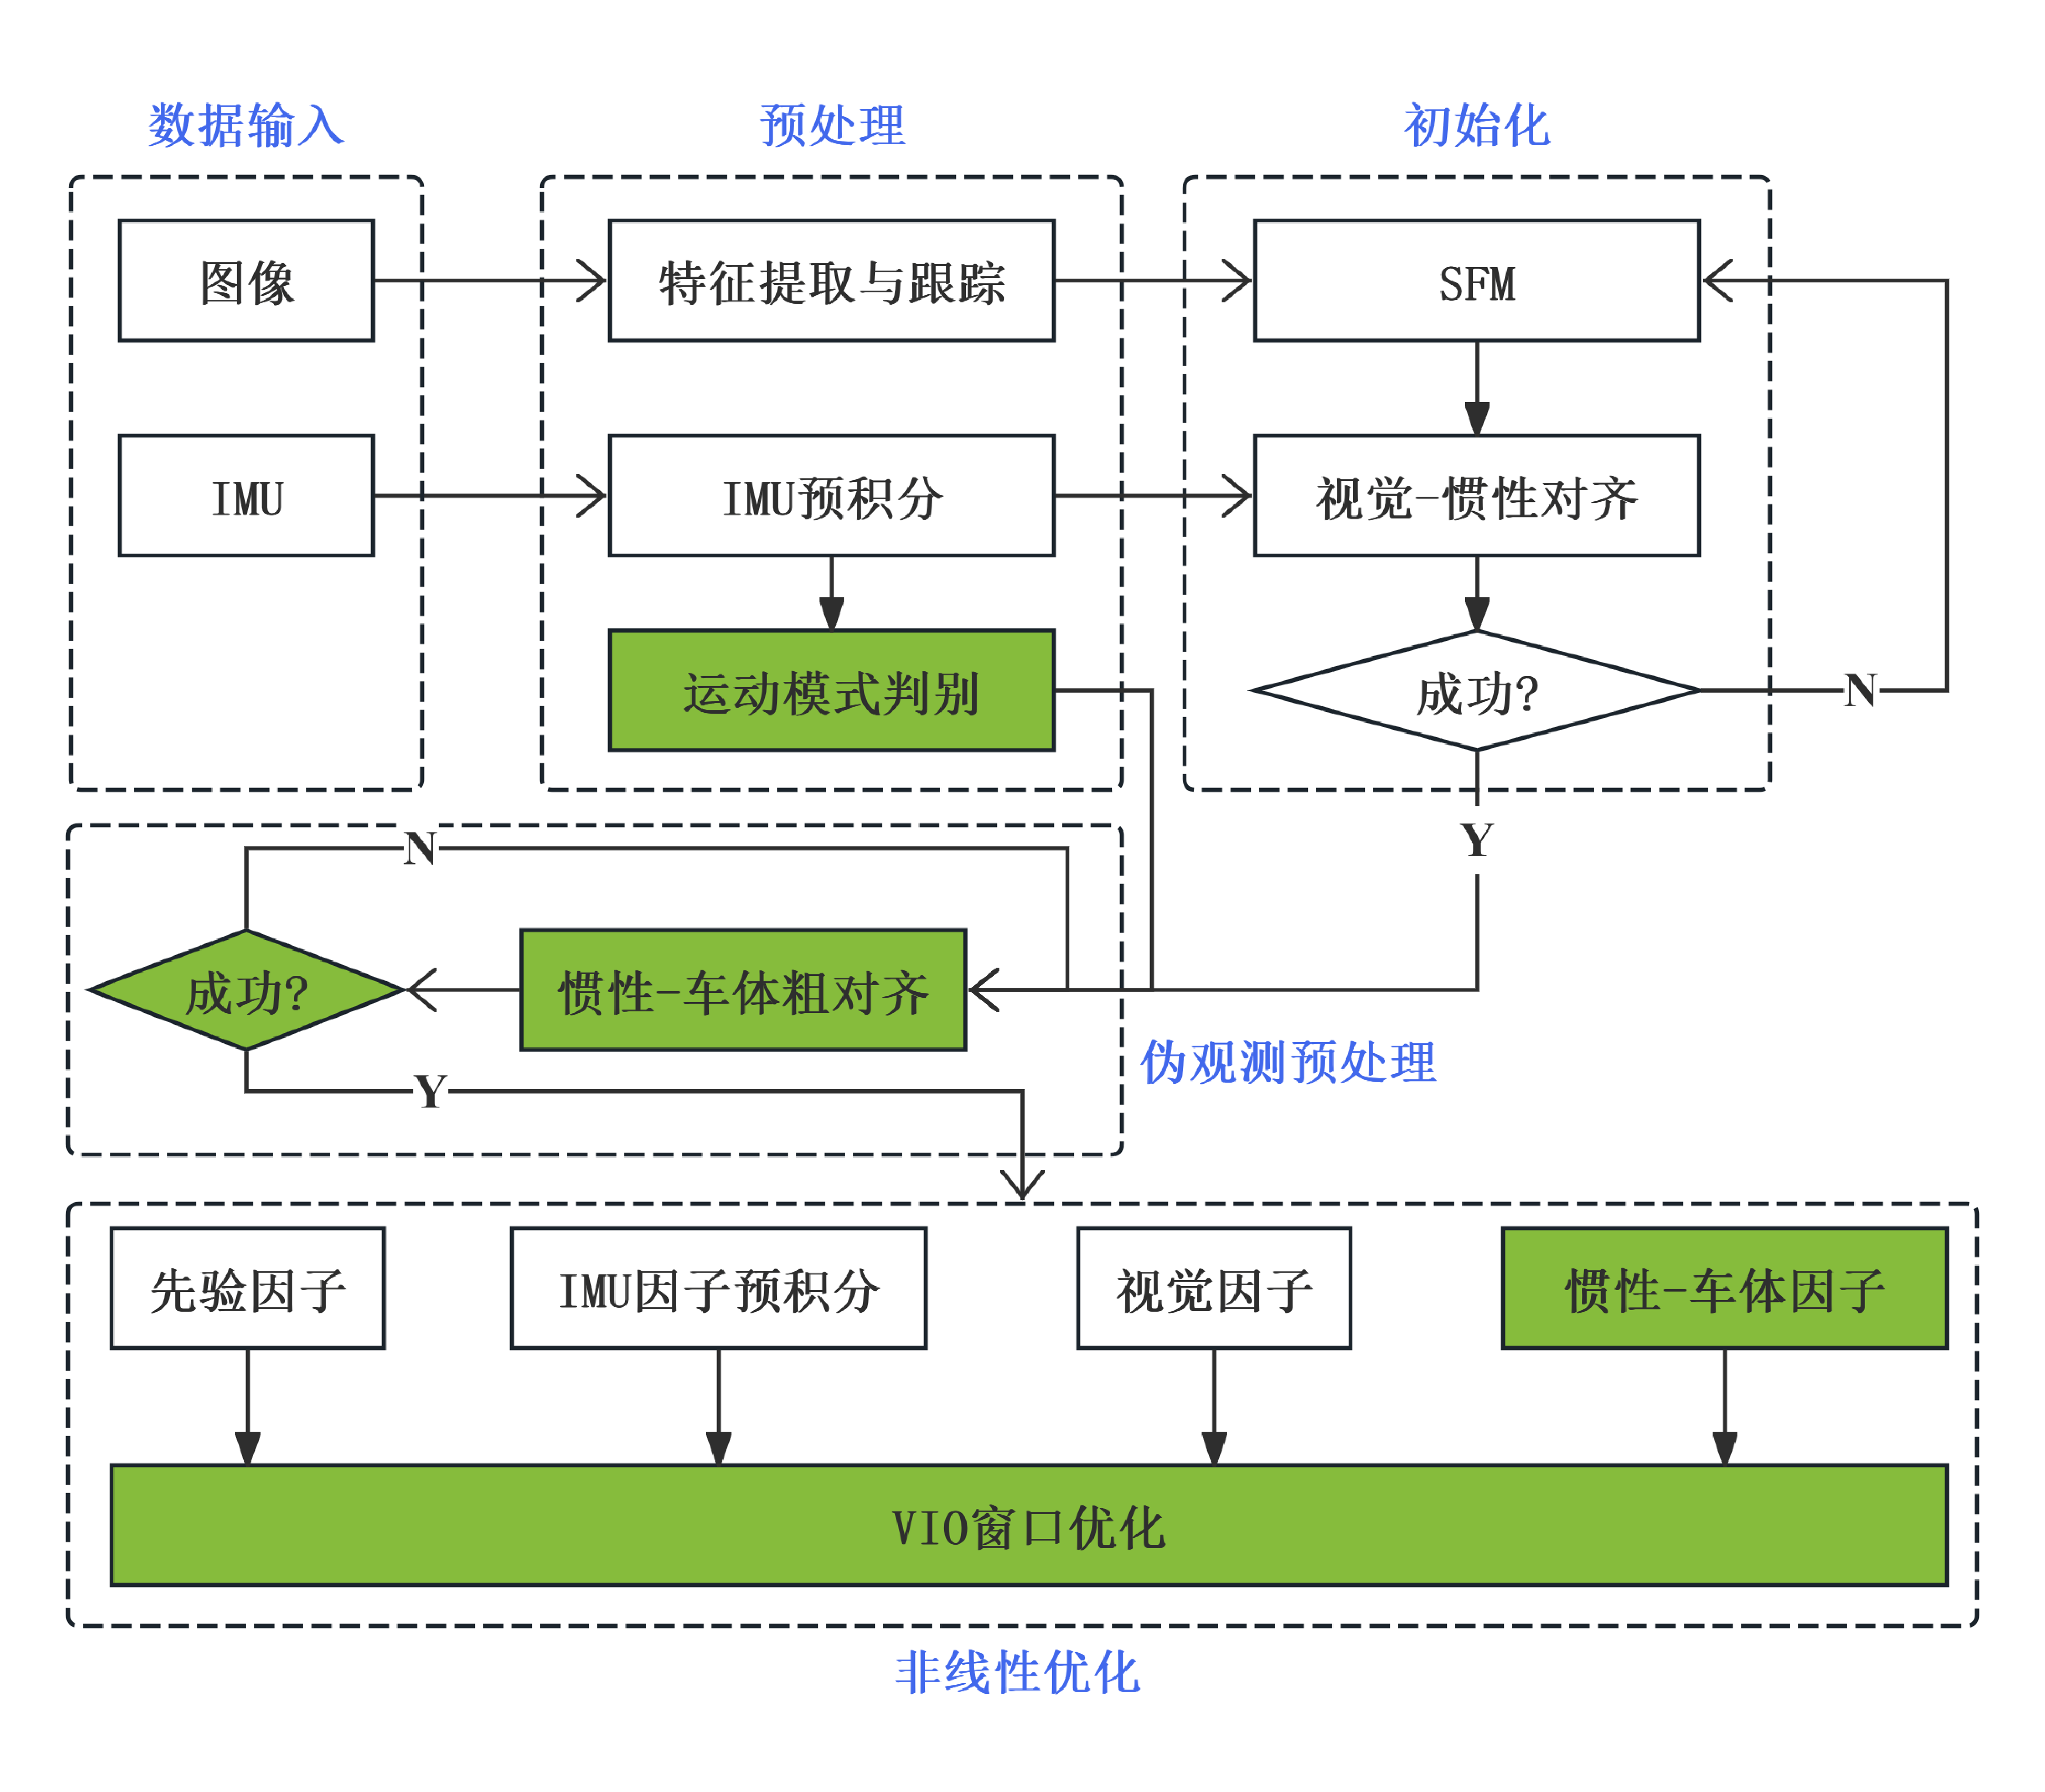
\includegraphics[width=0.9\linewidth]{VIO_pipeline.pdf}
  \caption{视觉惯性里程计框架}
  \label{fig:vio_pipeline}
\end{figure}

\section{车身状态判别}

根据对车身状态的分析,只有在车辆和机器人停止或直线行驶时,才能添加额外的约束。因此,需要在视觉惯性里程计中添加车身状态判别模块,以区分车辆的运动状态。以往的工作中,\citet{hu2020memsimu}使用传统的统计方法来判别车辆的直行、变道和转弯等状态;\citet{brossard2020ai}使用卷积神经网络(Convolutional Neural Network, CNN)来生成车身3个轴向的测量噪声,以此来间接判别车辆状态;\citet{huang2022vehicle}则使用时间卷积神经网络(Temporal Convolutional Neural Network, TCN)根据IMU观测值来接判别车辆的运动状态。然而,基于统计的判别方法需要事先采集IMU静止状态下的数据进行统计分析,不够灵活;基于CNN和TCN的方法针对每一条IMU数据进行判别,这在应用于高频率IMU(例如2000Hz及以上)时会造成极大的时延。针对以上问题,本文希望使用一种更加灵活,并且有望实时进行的方法来进行车身状态判别。

近年来,因为深度学习技术在泛化性能上展现出的优势,本文希望使用基于深度学习的方法来进行车身状态判别。在输入信息的选择上,为了使得深度神经网络能够与IMU的处理频率相匹配,就必须放弃以往逐条处理IMU数据的模式,转而寻找一种批量处理IMU数据的模式。在传统的视觉惯性里程计中,IMU数据的处理采用预积分的形式,简单来说,这是一种将IMU数据的采集频率与图像数据的采集频率相匹配的处理方式。在这种形势下,两张相邻时间图像之间的IMU数据会被整合为一个预积分因子,这样就可以将IMU数据的处理频率降低到与图像数据相同的频率,这个频率一般在10Hz到30Hz。在这个频率下,基于深度神经网络的方式是有望实时进行的,因此预积分因子内包含的IMU数据序列是一个理想的网络输入。

但是,如果选择预积分因子内的IMU数据序列作为网络输入,那么就会面临一个问题:因为IMU频率和相近频率不一定是整除关系,所以两帧图像之间的IMU序列并不等长。这就导致了擅长处理规整数据的CNN或者TCN并不适合处理预积分因子内的IMU数据序列。近年来,基于Transformer结构的神经网络在自然语言处理领域展现出了优异的性能,其注意力机制使得其能够处理任意长度的序列数据,所以也十分适合处理所有序列化的数据。基于此优势考虑,本文选择以Transformer结构为基础,设计一个用于车身状态判别的深度神经网络。

\subsection{网络预测状态}
对于网络的预测状态,本文选择对车身的$y$轴(车身前向)速度和$x$轴(车身横向)速度状态进行判别。用向量
\begin{equation}
  \symbf{z} = 
    \begin{bmatrix}
      z^{\rm FOR}\\
      z^{\rm LAT} 
    \end{bmatrix} \in \{0, 1\}^{2}
\end{equation}
来表示车身静止假设和直线行驶假设是否成立。其中$z^{\rm FOR}$指示车身静止假设是否成立,其分布为
\begin{equation}
  z^{\rm FOR} =
  \begin{cases}
    0, & \text{车辆静止假设不成立} \\
    1, & \text{车辆静止假设成立}
  \end{cases}.
\end{equation}
$z^{\rm FOR}$表示车身横向速度为0假设是否成立,其分布为
\begin{equation}
  z^{\rm LAT} =
  \begin{cases}
    0, & \text{车辆横向速度为0假设不成立} \\
    1, & \text{车辆横向速度为0假设成立}
  \end{cases}.
\end{equation}

\subsection{网络输入选择}
对于网络输入,本文使用一个预积分因子内的IMU数据序列作为网络输入。单条IMU采样数据包括加速度计读数$\hat{\symbf{a}}^b \in \mathbb{R}^3$和陀螺仪读数$\hat{\symbf{\omega}}^b \in \mathbb{R}^3$,两个读数的可以分解为:
\begin{equation}
\begin{aligned}
  &\hat{\symbf{a}}^b = \symbf{a}^b + \symbf{R}^{b}_{g}\cdot \symbf{g} + \symbf{b}_{a} + \symbf{n}_{a} \\
  &\hat{\symbf{\omega}}^b = \symbf{\omega}^b + \symbf{b}_{\omega} + \symbf{n}_{\omega} 
\end{aligned}
\end{equation}
其中$\symbf{a}^b, \symbf{\omega}^b$分别表示IMU此时真正的加速度和角速度,$\symbf{b}_{\omega}, \symbf{b}_{a}$分别表示陀螺仪和加速度计的零偏,$\symbf{n}_{\omega}, \symbf{n}_{a}$分别表示陀螺仪和加速度计的噪声,$\symbf{R}^{b}_{g}$表示此时全局坐标系到IMU体坐标系的旋转矩阵,$\symbf{g}$表示地球重力加速度。单条读数可以反映某一时刻的IMU运动情况,因此如果结合采样时间对IMU序列进行积分,就可以获得一段时间内的IMU运动情况,即旋转和位移。因此,使用IMU序列数据,理论上足以预测车身状态。实践中,本文将单条加速度计和单条陀螺仪读数拼接为一个6维向量,作为一条完整的IMU采样数据。在此之后,将预积分因子内的多条IMU采样数据拼接为一个矩阵$\symbf{X}\in \mathbb{R}^{n \times 6}$用以表示IMU数据序列,其中$\mathbb{R}^{n \times 6}$表示$\symbf{X}$由$n$条IMU读数组成。

\subsection{网络结构设计}
\begin{table}
  \centering
  \caption{车身判别网络设计参数}
  \begin{tabular}{ccccccc}
  \toprule
  层 & 层类型                 & 输入维度 & 特征维度 & 前馈层维度 & 头数 & 输出维度 \\
  \midrule
  1 & 全连接层                & 6    & 128  & N/A   & N/A & 128 \\
  2 & Transformer Encoder & 128  & 128  & 1024  & 8 & 128  \\
  3 & Transformer Encoder & 128  & 128  & 1024  & 8 & 128  \\
  4 & Transformer Decoder & 128  & 128  & 1024  & 8 & 128  \\
  5 & Transformer Decoder & 128  & 128  & 1024  & 8 & 128  \\
  6 & 全连接层                & 128  & 2    & N/A   & N/A & 2 \\
  \bottomrule
  \end{tabular}
  \label{tab:network}
\end{table}

对于网络结构,本文希望其能够输入一个可变形状矩阵$\symbf{X}$,稳定输出向量$\symbf{z}$。因此,本文使用了经典的Encoder-Decoder架构Transformer\cite{vaswani2017attention}:其网络的基本参数如表~\ref{tab:network} 所示。除了表中所示的神经网络层以外,本文网络中还有一个可训练参数$\symbf{q} \in \mathbb{R}^{128}$用于和两层Transformer Decoder进行交互已获得带有车身状态特征的向量$\symbf{q}' \in \mathbb{R}^{128}$,$\symbf{q}'$此后经全连接层获得预测向量$\symbf{y} \in \mathbb{R}^2$,$\symbf{y}$经过Sigmoid函数后得到预测的车身状态概率$\symbf{y} \in (0, 1)^2$。

\subsection{网络训练}

\renewcommand{\algorithmicrequire}{\textbf{输入:}\unskip}
\renewcommand{\algorithmicensure}{\textbf{输出:}\unskip}
\begin{algorithm}
  \caption{Generate training data and ground truth}
  \label{alg1}
  \small
  \begin{algorithmic}[1]
    \REQUIRE IMU时间戳序列$ts$, IMU采样数据序列$xs$, 车辆运动状态时间戳序列$vs$, 车辆位置状态序列$ps$, 车辆旋转状态序列$Rs$
    \ENSURE IMU数据序列列表$Xs$, 真值列表$zs$

    \STATE $vs$.insert(0, 0.0); $Xs \leftarrow []$; $Zs \leftarrow []$; $i \leftarrow 1$

    \WHILE{$i < $ len($vs$)}
      \STATE $j \leftarrow i-1$; $X \leftarrow []$; $z \leftarrow []$
      \WHILE{$ts[0] <= vs[j]$}
        \STATE $ts$.pop(0), $xs$.pop(0)
      \ENDWHILE
      \WHILE{$ts[0] <= vs[i]$}
        \STATE $X$.append($xs$.pop(0))
      \ENDWHILE
      \STATE $Xs$.append($X$)
      \IF{$ps[i] - ps[j] < {\epsilon}_p$}
        \STATE $z$.append(1)
      \ELSE
        \STATE $z$.append(0)
      \ENDIF
      \STATE $v \leftarrow Rs[j]^T \cdot Rs[i]$
      \IF{norm($v$)$<{\epsilon}_r$}
        \STATE $z$.append(1)
      \ELSE
        \STATE $z$.append(0)
      \ENDIF
      \STATE $zs$.append($z$)
    \ENDWHILE
  \end{algorithmic}
\end{algorithm}

对于网络训练,需要明确的问题主要包括数据清洗、预测真值生成、损失函数设计和训练策略。
在数据清洗方面,由于IMU采样数据包括加速度和角速度,这两类数据的数值分布有较大差异:角速度以$rad/s$为单位,一般是一个较小的数字,加速度以$m/s^2$为单位,其取值范围一般较大。因此如果使用原始数据作为网络输入,往往会造成网络训练的不稳定,因此本文使用归一化策略,将所有的IMU采样数据元素调整为值域在$(-1, 1)$之间:首先根据训练数据的分布特征计算IMU采样数据的均值$\symbf{\mu}\in \mathbb{R}^6$和逐元素标准差$\symbf{\sigma}\in \mathbb{R}^6$,然后对每一条IMU数据根据
\begin{equation}
  \symbf{x}' = \frac{\symbf{x} - \symbf{\mu}}{\symbf{\sigma}}
\end{equation}
进行转换。$\symbf{x}$是一条包涵加速度和角速度的IMU数据,除法是逐元素除法,可以在相同形状的的数据上进行操作。

在预测真值生成方面,本文需要使用到车辆的真实运动状态。具体来说,首先根据车辆的真实运动状态的更新频率切分IMU序列,然后根据车身运动状态自动生成真值$\symbf{z}$。根据对预设状态的分类,首先根据相对位置信息判断车辆是否静止,然后根据相对旋转判断车辆是否直线行驶,具体如算法~\ref{alg1} 所示,其中第16行即罗德里格斯旋转公式(Rodrigues' rotation formula)\cite{dai2015euler}将旋转矩阵转换为旋转向量,其具体过程详见附录~\ref{appendix:rodrigues},$\text{norm}(\cdot)$表示对向量取模操作。


在损失函数和训练策略方面,由于模型的最终输出会使用Sigmoid函数进行概率预测,相对应的损失函数选择二值交叉熵损失函数(Binary Cross Entropy, BCE)。在训练策略方面,本文使用Adam优化器\cite{kingma2014adam},学习率为$1e-4$,训练批次大小为8,训练轮数为100。此外,由于一般情况下车辆直行的情况比静止和转弯的情况要多,如图~\ref{fig:data_distrib} 所示,因此如果直接使用全部数据训练,则会导致样本分布的不均衡。为了解决这个问题,本文在数据采样方面使用了均衡策略:在训练的每个epoch中,以转弯和静止区间的并集数据量为基准,从直行数据中随机采样等量数据,然后与转弯和静止区间的并集数据合并。

\begin{figure}
  \centering
  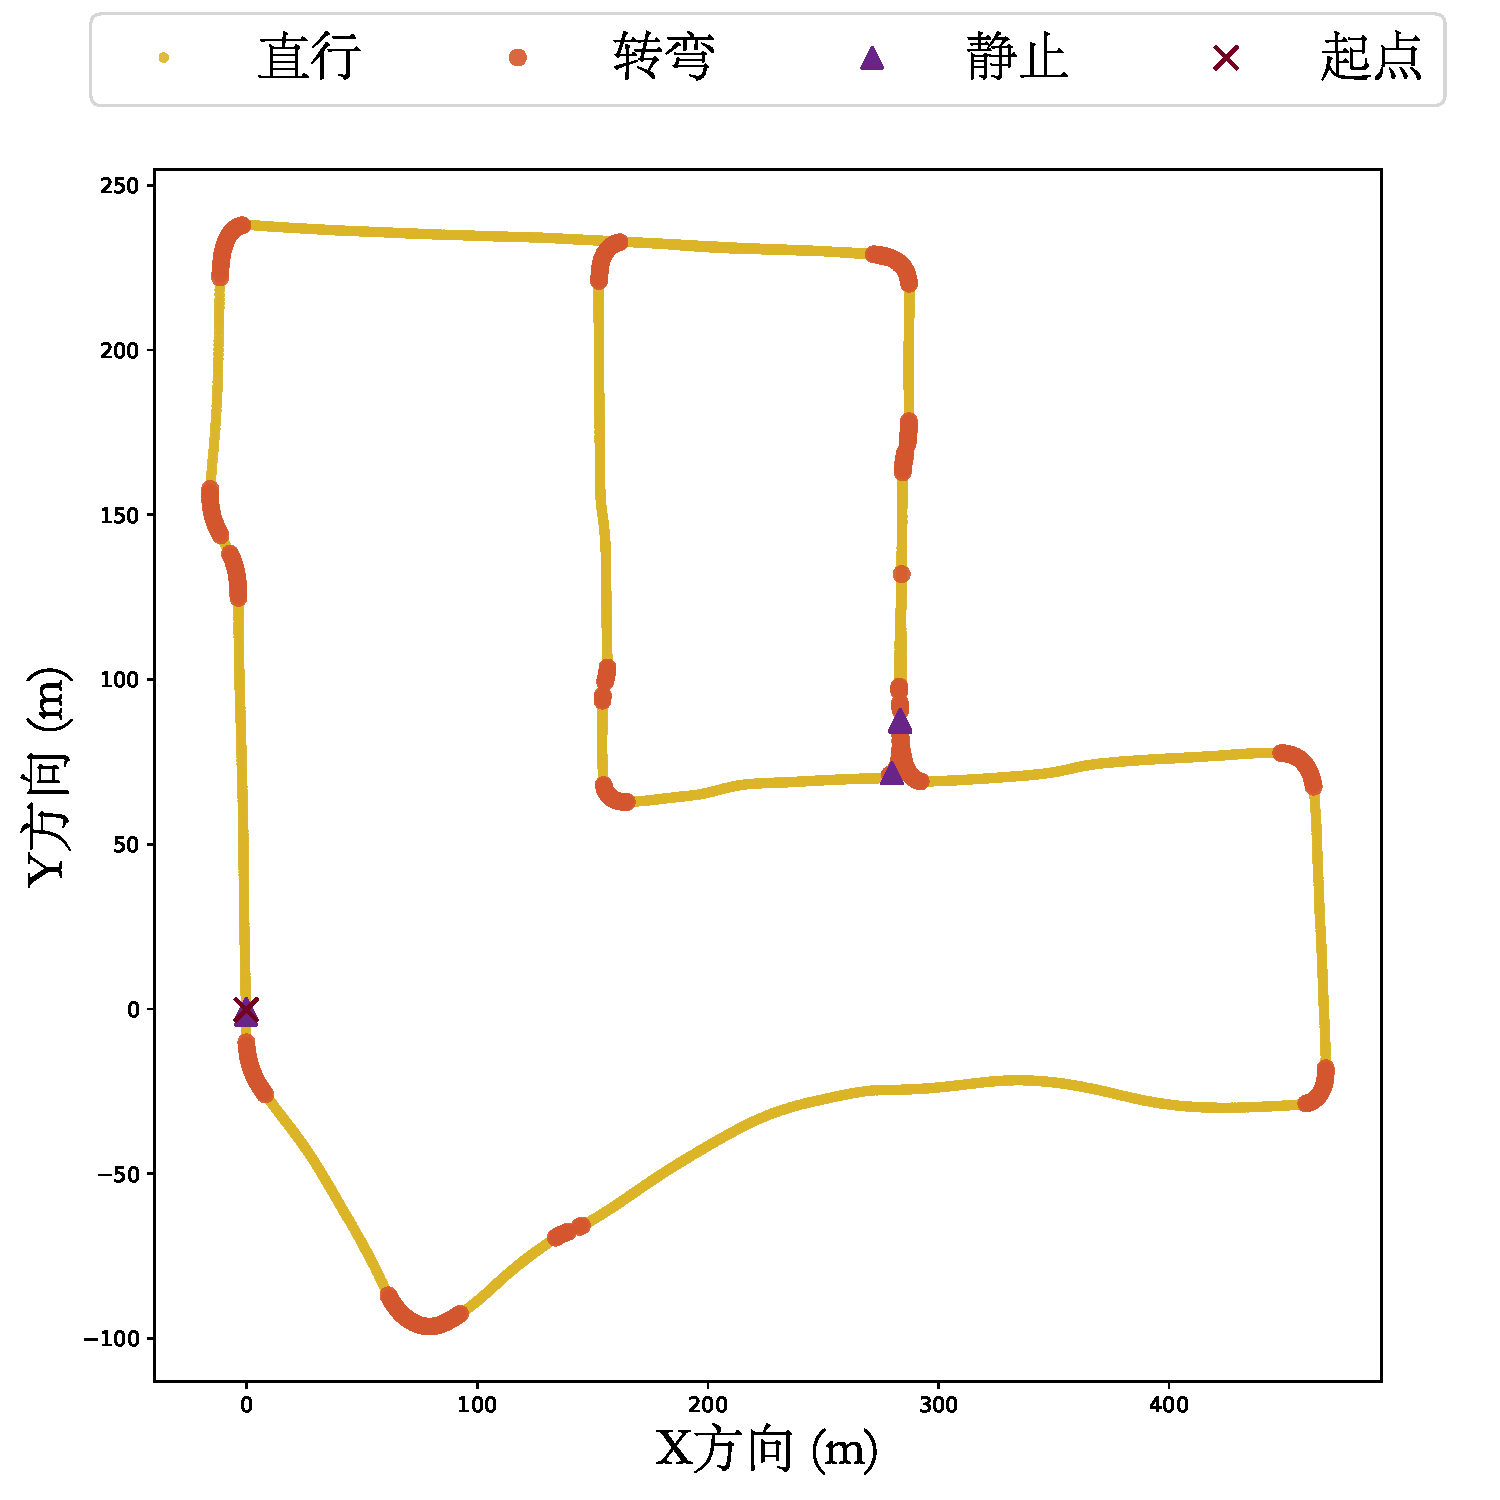
\includegraphics[width=0.47\linewidth]{distrib1.pdf}
  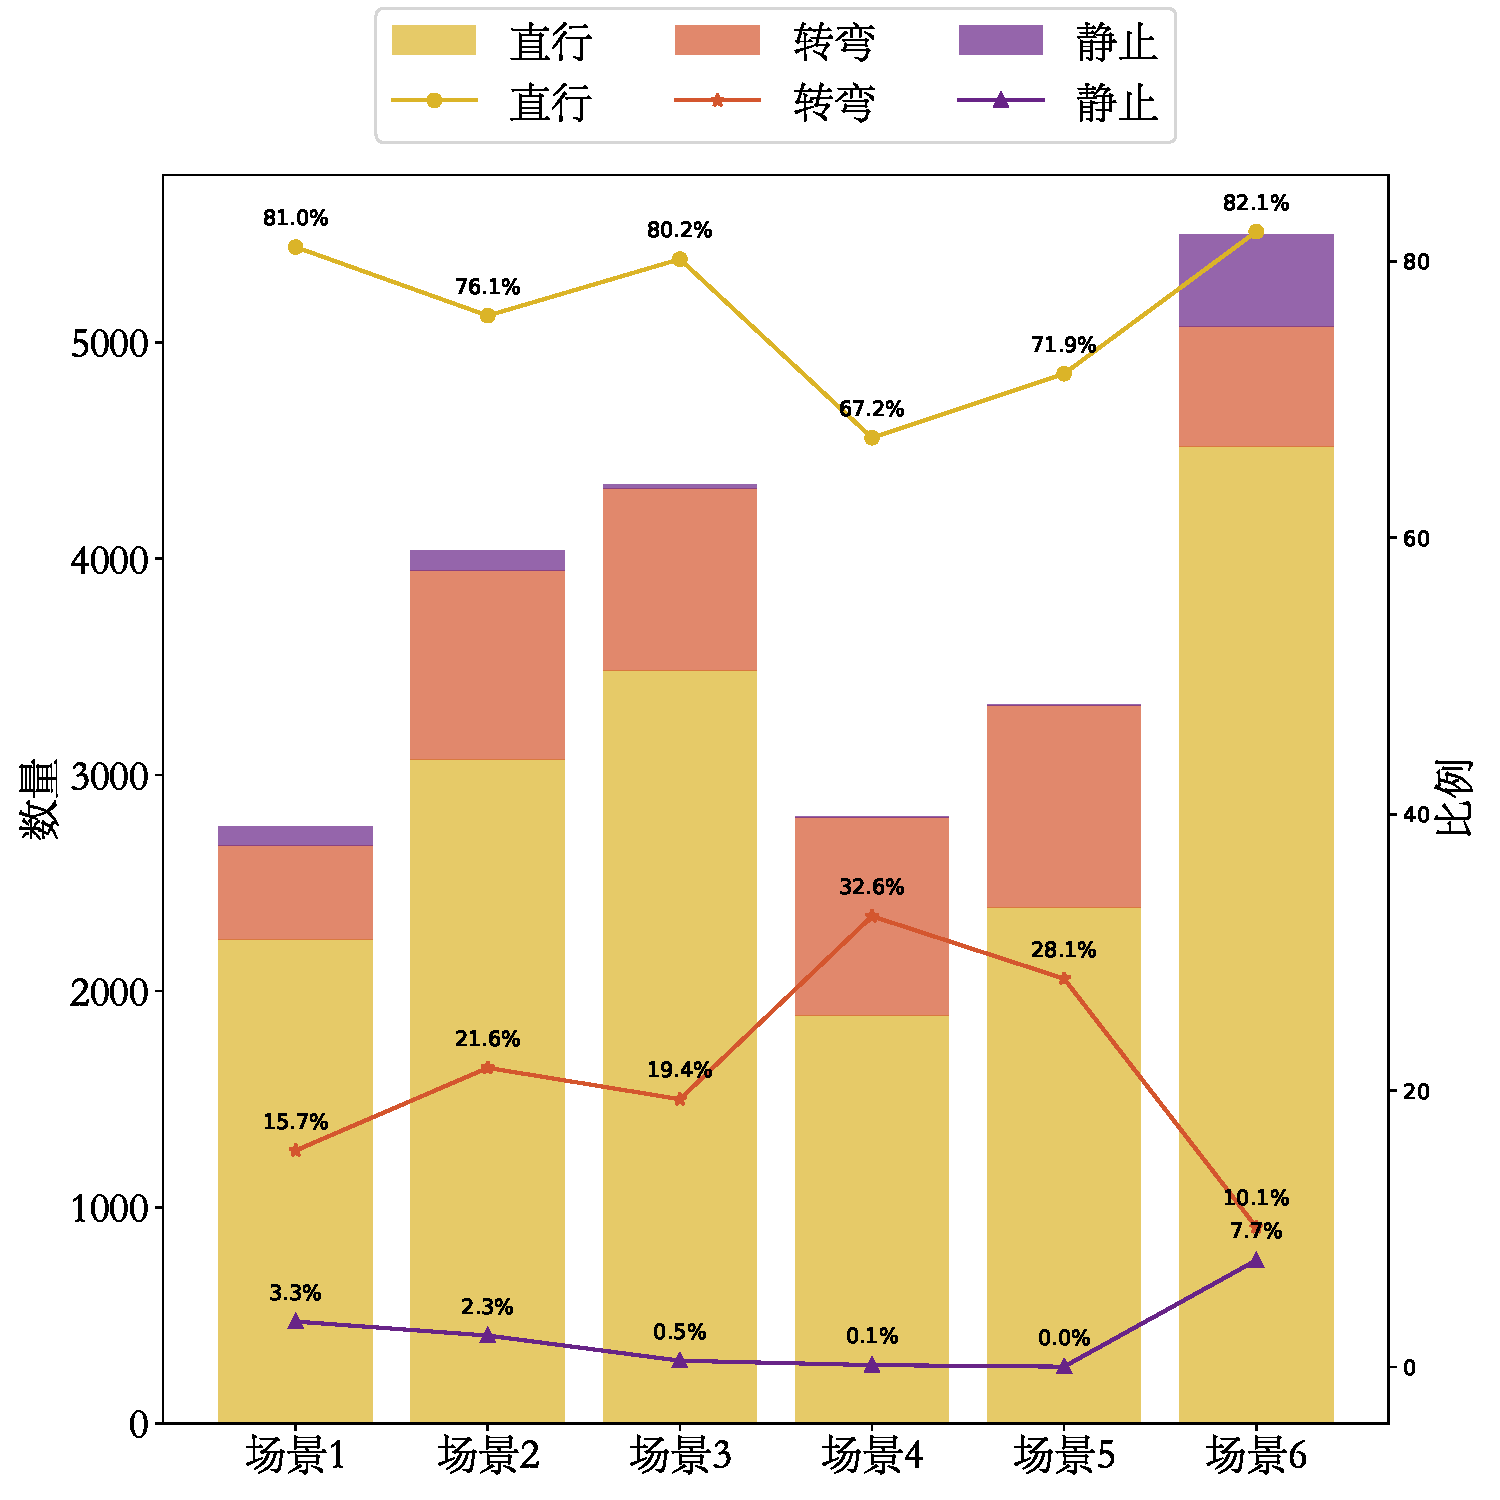
\includegraphics[width=0.47\linewidth]{hist.pdf}
  \caption{车身状态分布情况}
  \label{fig:data_distrib}
\end{figure}

\section{伪观测预处理}

伪观测可以为视觉惯性里程计增加一定的约束条件,但是其并不能直接使用,而是需要一定的预处理过程,其中最关键的就是惯性-车体粗对齐。如图~\ref{fig:vehicle} 中的坐标系示意图所示,车身坐标系和IMU体坐标系往往并不重合,有时甚至有较大的差距,而视觉惯性里程计中一般以IMU体坐标系作为姿态估计的基准坐标系。因此,如果使用车身坐标系的速度作为约束,就需要将车身坐标系的速度转换为IMU体坐标系的速度。这就需要进行惯性-车体粗对齐,即将车身坐标系的速度转换为IMU体坐标系的速度。一般来说,这个转换关系需要包含旋转和平移两种变换,但是考虑到车身整体的刚性结构,IMU与车身之间也是刚性连接,因此可以将车身坐标系与IMU体坐标系的原点等价为重合状态,在这种状态下可以只考虑车身坐标系与IMU坐标系之间的旋转关系。

在拥有状态判别,并且只考虑两坐标系之间旋转关系的情况下,求解车身坐标系和IMU体坐标系之间的关系还可以使用一些更强的先验知识:
\begin{enumerate}
  \item 在车辆直行的情况下,速度方向基本指向车身的前向,即车身坐标系的$y$轴;
  \item 在车辆直行的情况下,速度大小基本为合速度的模长。
\end{enumerate}
基于以上假设,可以使用以下方法求解车身坐标系和IMU体坐标之间的转换关系。

首先根据车身状态判别的结果,筛选直行时刻的IMU速度估计$\{\symbf{v}^o_{b_{j}}\}^n$,其中$\symbf{v}^o_{b_{j}}$表示第$j$时刻的IMU速度估计,$n$表示IMU速度估计的总数,然后使用视觉惯性里程计估计的车身姿态$\{ \symbf{R}_{b_{j}}^o\}^n$可以获得IMU体坐标系下的速度估计
\begin{equation}
  \{\symbf{v}^{b_{j}}\}^n = \{ {\symbf{R}_{b_{j}}^o}^{-1} \cdot \symbf{v}^o_{b_{j}} \}^n.
\end{equation}
又根据直线行驶时的车身假设可以获得此时车身坐标系下的速度为
\begin{equation}
  \{\symbf{v}^{v_{j}}\}^n = \{ \begin{bmatrix}
    0 \\
    \| \symbf{v}^{b_{j}} \| \\ 
    0
  \end{bmatrix}\}^n.
\end{equation}
此时,关于车体和IMU体坐标系之间的旋转关系$\symbf{R}_{b}^{v}$可以求解以下带有约束的优化问题获得:
\begin{equation}
\begin{aligned}
  &\min_{\symbf{R}_{b}^{v}} \symbf{J} = \frac{1}{2} \sum_{j=1}^{n} \| \symbf{v}^{v_{j}} - \symbf{R}_{b}^{v} \cdot \symbf{v}^{b_{j}} \|_2^2 \\
  \text{s.t.} & \quad {(\symbf{R}_{b}^{v})}^T \symbf{R}_{b}^{v} = \symbf{I}
\end{aligned},
\end{equation}
其中的约束条件是为了保证所求旋转矩阵是一个合法的旋转矩阵。针对上述优化问题,其求解过程如下:
\begin{align}
  2\symbf{J} &= \sum_{j=1}^{n} \| \symbf{v}^{v_{j}} - \symbf{R}_{b}^{v} \cdot \symbf{v}^{b_{j}} \|_2^2 \\ 
  &= \sum_{j=1}^{n} {(\symbf{v}^{v_{j}} - \symbf{R}_{b}^{v} \cdot \symbf{v}^{b_{j}})}^T \cdot {(\symbf{v}^{v_{j}} - \symbf{R}_{b}^{v} \cdot \symbf{v}^{b_{j}})} \\
  &= \sum_{j=1}^{n} {({\symbf{v}^{v_{j}}}^T - {\symbf{v}^{b_{j}}}^T \cdot {\symbf{R}_{b}^{v}}^T)} \cdot {(\symbf{v}^{v_{j}} - \symbf{R}_{b}^{v} \cdot \symbf{v}^{b_{j}})} \\
  &= \sum_{j=1}^{n} ({\symbf{v}^{v_{j}}}^T \cdot \symbf{v}^{v_{j}} - {\symbf{v}^{v_{j}}}^T \cdot \symbf{R}_{b}^{v} \cdot \symbf{v}^{b_{j}} - {\symbf{v}^{b_{j}}}^T \cdot {\symbf{R}_{b}^{v}}^T \cdot {\symbf{v}^{v_{j}}} + {\symbf{v}^{b_{j}}}^T \cdot {\symbf{R}_{b}^{v}}^T \cdot \symbf{R}_{b}^{v} \cdot \symbf{v}^{b_{j}}),
\end{align}
根据约束条件${(\symbf{R}_{b}^{v})}^T \symbf{R}_{b}^{v} = \symbf{I}$可得
\begin{align}
  2\symbf{J} &= \sum_{j=1}^{n} ({\symbf{v}^{v_{j}}}^T \cdot \symbf{v}^{v_{j}} - {\symbf{v}^{v_{j}}}^T \cdot \symbf{R}_{b}^{v} \cdot \symbf{v}^{b_{j}} - {\symbf{v}^{b_{j}}}^T \cdot {\symbf{R}_{b}^{v}}^T \cdot {\symbf{v}^{v_{j}}} + {\symbf{v}^{b_{j}}}^T \cdot \symbf{v}^{b_{j}}) \\ 
  &= \sum_{j=1}^{n} (\| \symbf{v}^{v_{j}} \|^2 - 2\cdot {\symbf{v}^{v_{j}}}^T \cdot \symbf{R}_{b}^{v} \cdot \symbf{v}^{b_{j}} + \| \symbf{v}^{b_{j}} \|^2) \\
  &= \sum_{j=1}^{n} (\| \symbf{v}^{v_{j}} \|^2 + \| \symbf{v}^{b_{j}} \|^2) - 2 \sum_{j=1}^{n} {\symbf{v}^{v_{j}}}^T \cdot \symbf{R}_{b}^{v} \cdot \symbf{v}^{b_{j}},
\end{align}
可以观察到此时$\symbf{J}$的最小化与前一常数项无关,仅与后项带$\symbf{R}_b^v$的项有关,因此可以将$\symbf{J}$的最小化问题转化为最大化后一项,即
\begin{equation}
  \max_{\symbf{R}_{b}^{v}} \symbf{J}' = \sum_{j=1}^{n} {\symbf{v}^{v_{j}}}^T \cdot \symbf{R}_{b}^{v} \cdot \symbf{v}^{b_{j}}.
\label{eq:max}
\end{equation}
注意到
\begin{align}
  \sum_{j=1}^{n} {\symbf{v}^{v_{j}}}^T \cdot \symbf{R}_{b}^{v} \cdot \symbf{v}^{b_{j}} &= \text{trace}({\symbf{V}^{v}}^T \cdot \symbf{R}_{b}^{v} \cdot \symbf{V}^{b}) \\ 
  &= \text{trace}( \symbf{R}_{b}^{v} \cdot \symbf{V}^{b} \cdot {\symbf{V}^{v}}^T), \label{eq:trace}
\end{align}
其中$\symbf{V}^{b}, {\symbf{V}^{v}}^T$分别是$\{\symbf{v}^{b_{j}}\}^n,\{\symbf{v}^{v_{j}}\}^n$序列的协方差矩阵。对$\symbf{V}^{b} \cdot {\symbf{V}^{v}}^T$进行奇异值分解(Singular Value Decomposition, SVD)可以获得
\begin{equation}
  \symbf{V}^{b} \cdot {\symbf{V}^{v}}^T = \symbf{U} \cdot \symbf{\Sigma} \cdot \symbf{V}^T,
\label{eq:svd}
\end{equation}
因此可以对式~\eqref{eq:trace}进行变换得到
\begin{align}
  \text{trace}( \symbf{R}_{b}^{v} \cdot \symbf{V}^{b} \cdot {\symbf{V}^{v}}^T) &= \text{trace}(\symbf{R}_{b}^{v} \cdot \symbf{U} \cdot \symbf{\Sigma} \cdot \symbf{V}^T) \\
  &= \text{trace}(\symbf{\Sigma} \cdot \symbf{V}^T \cdot \symbf{R}_{b}^{v} \cdot \symbf{U}),
\end{align}
其中$\symbf{V}^T \cdot \symbf{R}_{b}^{v} \cdot \symbf{U}$为三个正交矩阵的乘积,因此仍是一个正交矩阵,而$\symbf{\Sigma}$为对角矩阵。根据正交矩阵的性质可知其内部所有元素均小于1(因为正交矩阵的行列式为1),所以对于$\text{trace}(\symbf{\Sigma} \cdot \symbf{V}^T \cdot \symbf{R}_{b}^{v} \cdot \symbf{U})$来说,其取得最大值时即$\symbf{V}^T \cdot \symbf{R}_{b}^{v} \cdot \symbf{U}$为单位矩阵。结合式~\eqref{eq:max},式~\eqref{eq:trace},式~\eqref{eq:svd}可知,最大化$\symbf{J}'$时即
\begin{equation}
  \symbf{R}_{b}^{v} = \symbf{V} \cdot \symbf{U}^T.
\end{equation}
此时获得的$\symbf{R}_{b}^{v}$可能会因为存在噪声等原因而并不精确,但此过程仅为粗对齐,所以精度误差有一定的容忍,后续在非线性优化部分仍会对此参数进行持续优化。

\section{非线性优化}
经过车身状态判别和惯性-车体粗对齐之后,还需要将伪观测相关的两个因子加入到VIO的窗口优化中,才能发挥伪观测约束对于整个系统的提升作用。由于伪观测约束是在原有视觉惯性里程计的优化项上添加,因此描述伪观测约束的相关因子,必须了解视觉惯性里程计的状态估计量及相关约束。

本文的视觉惯性里程计的估计量可以表示为
\begin{equation}
\begin{aligned}
  \mathcal{X} &= \begin{bmatrix} \symbf{x}_0, \symbf{x}_1, \dots, \symbf{x}_n, \symbf{x}_c^b, \symbf{q}_b^v, \lambda_0, \lambda_1, \dots, \lambda_m \end{bmatrix} \\
  \symbf{x}_k &= \begin{bmatrix} \symbf{p}_{b_{k}}^o, \symbf{v}_{b_{k}}^o, \symbf{q}_{b_{k}}^o, \symbf{b}_a, \symbf{b}_{\omega} \end{bmatrix} \\
  \symbf{x}_c^b &= \begin{bmatrix} \symbf{q}_{c}^b, \symbf{q}_{c}^b \end{bmatrix}
\end{aligned},
\end{equation}
其中$\symbf{x}_k$表示第$k$帧时刻的IMU姿态,$\symbf{x}_c^b$表示相机到IMU的外参,$\symbf{q}_b^v$表示IMU到车身的外参,$\lambda_k$表示第$k$帧相机的特征点深度。$\symbf{q}_b^v$是惯性-车体因子,其表示IMU体坐标系到车身坐标系的旋转关系。

根据以上的状态估计量,可以得到视觉惯性里程计的优化目标函数
\begin{equation}
  \min_{\mathcal{X}} 
  \begin{Bmatrix} 
  \| \symbf{r}_p - \symbf{H}_p \cdot \mathcal{X} \|^2 + \sum_{k\in\mathcal{B}} \| \symbf{r}'_{\mathcal{B}}(\hat{\symbf{z}}_{b_k}^{b_{k+1}}, \mathcal{X}) \|^2_{\symbf{P}_{b_k}^{b_{k+1}}}
  + \sum_{(l,j)\in\mathcal{C}} \rho(\| \symbf{r}_{\mathcal{C}}(\hat{\symbf{z}}_{l}^{c_j}, \mathcal{X}) \|^2_{\symbf{P}_{l}^{c_j}}) \end{Bmatrix},
\end{equation}
其中$\symbf{r}_p, \symbf{H}_p$代表与边缘化相关的观测与矩阵,$\symbf{r}_{\mathcal{C}}$代表视觉观测的残差函数,$\symbf{r}'_{\mathcal{B}}$是本文提出的、增加了伪观测约束的IMU残差函数,$\symbf{P}_{l}^{c_j}$代表视觉观测的协方差矩阵,$\symbf{P}_{b_k}^{b_{k+1}}$代表伪观测约束的协方差矩阵,$\mathcal{B}$表示存在IMU残差的时刻集合,$\mathcal{C}$则表示地图点和视觉观测的匹配集合。$\symbf{r}'_{\mathcal{B}}$具体可以表示为
\begin{equation}
  \symbf{r}'_{\mathcal{B}}(\hat{\symbf{z}}_{b_k}^{b_{k+1}}, \mathcal{X}) = 
  \begin{bmatrix} 
    \symbf{R}_o^{b_k} \cdot (\symbf{p}_{b_{k+1}}^o -\symbf{p}_{b_k}^o-\symbf{v}_{b_k}^o\cdot\Delta t_k + \frac{1}{2}\symbf{g}^o{\Delta t_k}^2) - \hat{\symbf{\alpha}}_{b_{k+1}}^{b_k} \\
    \symbf{R}_o^{b_k} \cdot (\symbf{v}_{b_{k+1}}^o - \symbf{v}_{b_k}^o + \symbf{g}^o\Delta t_k) - \hat{\symbf{\beta}}_{b_{k+1}}^{b_k} \\
    2[{\symbf{q}^o_{b_k}}^{-1}\otimes\symbf{q}_{b_{k+1}}^o \otimes \hat{\symbf{\gamma}}_{b_{k+1}}^{b_k}]_{xyz} \\
    \symbf{b}_{ab_{k+1}} - \symbf{b}_{ab_{k}} \\
    \symbf{b}_{\omega b_{k+1}} - \symbf{b}_{\omega b_{k}} \\
    \symbf{A} \cdot \symbf{R}_b^v \cdot {\symbf{R}_{b_k}^o}^{-1} \cdot \symbf{v}_{b_k}^o
  \end{bmatrix},
  \label{eq:imu_residual}
\end{equation}
其中$\Delta t_k$表示时间间隔,$\symbf{g}^o$表示VIO世界坐标系下的重力向量,$\hat{\symbf{\alpha}}_{b_{k+1}}^{b_k}, \hat{\symbf{\beta}}_{b_{k+1}}^{b_k}, \hat{\symbf{\gamma}}_{b_{k+1}}^{b_k}$分别表示相对位移、相对速度和相对旋转的预积分观测值,其具体表示参考\citet{qin2018vins}的工作。IMU残差函数的最后一项是相较于经典视觉惯性里程计而增加的速度伪观测约束。$A$是一个指示函数,其取值根据车身状态判别的结果取值
\begin{equation}
  A = 
  \begin{cases}
    \begin{bmatrix} \symbf{e_1}, \symbf{e_2}, \symbf{e_3}  \end{bmatrix}, \symbf{y}^{FOR} = 1 \\
    \begin{bmatrix} \symbf{0}, \symbf{e_2}, \symbf{e_3}  \end{bmatrix}, \symbf{y}^{LAT} = 1 \\
    \begin{bmatrix} \symbf{0}, \symbf{0}, \symbf{0}  \end{bmatrix}, \text{Otherwise}
  \end{cases}.
\end{equation}
其中$\symbf{e}_i$表示单位矩阵的第$i$列向量,$\symbf{y}^{FOR}, \symbf{y}^{LAT}$分别表示预测的车辆前进和横向的状态。

若使用伪观测约束,需要使用其相对于各估计量的雅可比矩阵。为了简化表达,本处使用$\symbf{r}'_{\mathcal{B}}$代表IMU残差函数中的伪观测约束,即式~\eqref{eq:imu_residual}的最后一项。首先给出速度伪观测约束相对于状态量$\symbf{v}_{b_{k}}^o$的雅可比矩阵
\begin{equation}
  \frac{\partial \symbf{r}'_{\mathcal{B}}}{\partial \symbf{v}_{b_{k}}^o} = \symbf{A} \cdot \symbf{R}_b^v \cdot {\symbf{R}_{b_k}^o}^{-1}.
\label{eq:JrJv}
\end{equation}
对于$\symbf{q}_{b_{k}}^o$的雅可比矩阵,约束中并没有直接使用四元数$\symbf{q}_{b_{k}}^o$,而是使用等价的旋转矩阵$\symbf{R}_{b_{k}}^o$,避免了四元数运算$\otimes$的繁琐使用。求导方式本文选择使用扰动模型\cite{imu_preintegration}进行,假设旋转的扰动值为$\symbf{\varphi } \in \mathbb{R}^3$(对于四元数和旋转矩阵有同样的效果),则:
\begin{align}
  \frac{\partial \symbf{r}'_{\mathcal{B}}}{\partial \symbf{q}_{b_{k}}^o} &\triangleq  \frac{\partial \symbf{r}'_{\mathcal{B}}}{\partial \symbf{\varphi }} \\
  &= \lim\limits_{\symbf{\varphi } \to \symbf{0}} \frac{\symbf{A} \cdot \symbf{R}_b^v \cdot {\text{exp}(\symbf{\varphi }^{\land}) \cdot {\symbf{R}_{b_k}^o}^{-1}} \cdot \symbf{v}_{b_k}^o - \symbf{A} \cdot \symbf{R}_b^v \cdot {{\symbf{R}_{b_k}^o}^{-1}} \cdot \symbf{v}_{b_k}^o}{\symbf{\varphi }} \\
  &= \lim\limits_{\symbf{\varphi } \to \symbf{0}} \frac{\symbf{A} \cdot \symbf{R}_b^v \cdot {\text{exp}(\symbf{\varphi }^{\land}) \cdot \symbf{R}^{b_k}_o} \cdot \symbf{v}_{b_k}^o - \symbf{A} \cdot \symbf{R}_b^v \cdot {\symbf{R}^{b_k}_o} \cdot \symbf{v}_{b_k}^o}{\symbf{\varphi }} \\
  &= \lim\limits_{\symbf{\varphi } \to \symbf{0}} \frac{\symbf{A} \cdot \symbf{R}_b^v \cdot {[(\symbf{I} + \symbf{\varphi }^{\land}) \cdot \symbf{R}^{b_k}_o]} \cdot \symbf{v}_{b_k}^o - \symbf{A} \cdot \symbf{R}_b^v \cdot {\symbf{R}^{b_k}_o} \cdot \symbf{v}_{b_k}^o}{\symbf{\varphi }} \\
  &= \lim\limits_{\symbf{\varphi } \to \symbf{0}} \frac{\symbf{A} \cdot \symbf{R}_b^v \cdot {({\symbf{R}^{b_k}_o} + \symbf{\varphi }^{\land} \cdot \symbf{R}^{b_k}_o)} \cdot \symbf{v}_{b_k}^o - \symbf{A} \cdot \symbf{R}_b^v \cdot {\symbf{R}^{b_k}_o} \cdot \symbf{v}_{b_k}^o}{\symbf{\varphi }} \\
  &= \lim\limits_{\symbf{\varphi } \to \symbf{0}} \frac{\symbf{A} \cdot \symbf{R}_b^v \cdot {\symbf{\varphi }^{\land} \cdot \symbf{R}^{b_k}_o} \cdot \symbf{v}_{b_k}^o}{\symbf{\varphi }}
  = \lim\limits_{\symbf{\varphi } \to \symbf{0}} \frac{-\symbf{A} \cdot \symbf{R}_b^v \cdot ({\symbf{R}^{b_k}_o} \cdot \symbf{v}_{b_k}^{o})^{\land} \cdot \symbf{\varphi}}{\symbf{\varphi }} \\
  &= -\symbf{A} \cdot \symbf{R}_b^v \cdot ({\symbf{R}^{b_k}_o} \cdot \symbf{v}_{b_k}^{o})^{\land}
  = -\symbf{A} \cdot \symbf{R}_b^v \cdot ({\symbf{R}_{b_k}^o}^{-1} \cdot \symbf{v}_{b_k}^{o})^{\land}, \label{eq:JrJqb}
\end{align}
其中${\land}$表示将一个向量转换为反对称矩阵的函数,在推导中直接使用了近似
\begin{equation}
  \text{exp}(\symbf{\varphi }^{\land}) \approx \symbf{I} + \symbf{\varphi }^{\land}.
\end{equation}
和反对称矩阵的乘法交换规律
\begin{equation}
  \symbf{a}^{\land} \cdot \symbf{b} = -\symbf{b}^{\land} \cdot \symbf{a}.
\end{equation}
同理可得伪观测约束关于惯性-车体因子的雅可比矩阵:
\begin{equation}
  \frac{\partial \symbf{r}'_{\mathcal{B}}}{\partial \symbf{q}_{b}^v} = -\symbf{A} \cdot (\symbf{R}_b^v \cdot {\symbf{R}_{b_k}^o}^{-1} \cdot \symbf{v}_{b_k}^o)^{\land}.
  \label{eq:JrJqv}
\end{equation}
至此已经给出了速度伪观测对于估计量的雅可比矩阵。根据雅可比矩阵,使用高斯牛顿法或者列文伯格-马夸尔特法进行非线性优化,以获得最终的状态估计量。

\section{本章总结}
本章主要介绍了固定路线定位系统中的视觉惯性里程计设计。整体设计考虑了车辆或轮式机器人的特殊运动状态,首先借助深度学习技术对车辆的运动状态进行判别,这一部分包括了网络设计和详细的训练过程;然后根据判别结果进行伪观测预处理,这一部分主要是使用视觉惯性里程计本身估计的速度和假设的车身状态进行粗对齐;最后将伪观测约束和惯性-车体因子加入到视觉惯性里程计的非线性优化中,以提高定位的精度。